\documentclass[11pt,fleqn,twoside]{article}
\usepackage{makeidx}
\makeindex
\usepackage{palatino} %or {times} etc
\usepackage{plain} %bibliography style 
\usepackage{amsmath} %math fonts - just in case
\usepackage{amsfonts} %math fonts
\usepackage{amssymb} %math fonts
\usepackage{lastpage} %for footer page numbers
\usepackage{fancyhdr} %header and footer package
\usepackage{mmpv2} 
\usepackage{url}
\usepackage{array}
\usepackage{graphicx}
\usepackage{float}

\usepackage[
	pdfborder={0 0 0},
	pdfstartview={FitH},
	plainpages=false,
	pdfpagelabels,
	bookmarksopen=true,
	bookmarksopenlevel=1
	]{hyperref}

% the following packages are used for citations - You only need to include one. 
%
% Use the cite package if you are using the numeric style (e.g. IEEEannot). 
% Use the natbib package if you are using the author-date style (e.g. authordate2annot). 
% Only use one of these and comment out the other one. 
\usepackage{cite}
%\usepackage{natbib}

\begin{document}

\name{Emanuil Tolev}
\userid{eet9}
\projecttitle{Sharing and mapping out scholarly funding opportunities}
\projecttitlememoir{Sharing and mapping out scholarly funding opportunities} %same as the project title or abridged version for page header
\reporttitle{Progress Report}
\version{1.0}
\docstatus{Release}
\modulecode{CS39440}
\supervisor{Reyer Zwiggelaar} % e.g. Neil Taylor
\supervisorid{rrz}
\wordcount{4266}

%optional - comment out next line to use current date for the document
%\documentdate{26th October 2011} 
\mmp

\setcounter{tocdepth}{3} %set required number of level in table of contents
\tableofcontents

\newpage

%==============================================================================
\section{Project Summary}
%==============================================================================
%This section should explain what your project is, identify how it relates to existing work and identify the project goals.
% 1000 words


%You should introduce your project and provide an overall summary of what your project is about and why you find it interesting, challenging and worthwhile.
\subsection{Scholarly funding opportunities}
This project deals with an important bit of the infrastructure of scholarship - namely, the money it relies upon. ``Scholarship'' in this case (and throughout this document) refers to the human endeavours in the fields of the Humanities(e.g. arts), Social Sciences (e.g. law) and Science (e.g. biology, computer science).

The problem is that scholarly funding has a very peculiar system which has evolved over time from a series of ad-hoc changes to the way money is distributed in society. There is no easy way to track money - where it gets allocated to, what fields (or even topics) within scholarship get funded more than others. This has resulted in several problems:

\subsubsection{Funders}
There is no easy way for people who wish to fund scholarly endeavours to advertise their funding to a lot of scholars at once, getting a higher chance of the ``perfect'' researcher/problem fit.

Certain ad-hoc channels have evolved around this problem - for example, scholars interested in a funder's sphere can subscribe to their e-mail list. There are problems with this - the most obvious one is scholars having to subscribe to all the funders they might be interested in. While this sort of works for national funding bodies like the UK Research Councils, there are many more private funders - various non-profit and/or Non-Governmental Organisations and even private companies. A cross-disciplinary funding opportunity would have to be advertised across multiple channels, which would take time/effort on the part of funders therefore making such opportunities costlier to set up.

It also fails fantastically when it comes to the globalisation of scholarship. There are only two ways to get to know about funds coming from the other side of the world:
\begin{enumerate}
	\item directly: be subscribed to that particular funder's news (the number of funders has not been estimated globally to the best of the author's knowledge, not to mention the huge variety of forms which news feeds take - from RSS through e-mail to just publishing on a website somewhere).
	\item indirectly: hear about the opportunity from others. ``Others'' could mean colleagues - research development officers, other scholars - but these people have to be directly or indirectly related to the funding source. The funder will only reach a very small subset of the world's scholars directly, however, and this is crucial for a network model.
\end{enumerate}

The other currently possible meaning of ``Others'' is commercial companies who collect scholarly funding information, package it into databases with a front-end and sell it to research institutions. While the author is not against making a profit out of information, there has been overwhelming evidence in the past two decades that commercially exploiting information \emph{by virtue of hoarding it and then restricting access to it} is not a good strategy for anybody but the hoarder.

\subsubsection{The value of Openness in scholarship and elsewhere}
The Free Software, Open Source and more recently, Open Knowledge (which Open Access is a part of) movements have all demonstrated that the value of information can be greatly multiplied simply by having more people access it, reuse it and even be creative with it (e.g. visualise or summarise). The Open Knowledge Foundation argues this \cite{okfn-vision}. Seminal works like ``The Cathedral and the Bazaar'' \cite{catb} have also argued this.

Governments seem to have grasped the benefits as well. The UK Government has mandated that all research funded with public money (which is a lot in the UK - almost everything through the seven Research Councils) should be published as Open Access by 2014 \cite{guardian-ukgov-oa2014}. It has also funded initiatives such as Open UK governmental data in the form of data.gov.uk \cite{open-uk-gov-data} and the recent Finch report \cite{guardian-finch} \cite{finch}.

Private organisations are not far behind and may in fact be leading the way - one of the largest funders of science in the UK and around the world, the Wellcome Trust, has had a progressive and strict Open Access policy since 2006 \cite{wellcome-oa}.

\subsubsection{Scholars}
Openness is recognised as beneficial - and many scholars are supposed to be able to benefit from having access to all this scholarship for free instead of having the libraries pay extortionate amounts to academic publishers. The very essence of scholarship is building on what has been discovered before.

However, while previous knowledge is a core requirement of science, sustenance is a very core human requirement, and in the modern world, this often translates to salaries \emph{and} (sometimes ``\emph{or}'') grant money, at least for scholars. Why should \emph{this} information be commercially exploited for the benefit of a few corporations when it could be used to better (globally) connect the minds to the money, to put it bluntly?

There is another point - information about funding opportunities may be available but may be too generic or hidden beyond layers and layers of website navigation, reflecting the mental model of the funding organisation instead of the mental model of the researcher (RCUK are a case in point \cite{rcuk-home}). Thus, the goal of this project from the perspective of scholars can be summarised as ``bringing it together''.

\subsection{The project}
This project is about making an open-source web application named ``FundFind'' which lets stakeholders (just the scholars at first) share information about funding opportunities under open terms (the Open Definition defines ``open'' well \cite{od}).

Follow-up work may increase this scope to include funding organisations or governments - they will already be able to submit funding information directly to a centrally hosted instance of the software produced by this project, but they will probably have special requirements related to this.

The project does include functionality to allow scholars to access the information, and allow developers / journalists / analysts and other stakeholders to analyse and mash up the information.

\subsection{Existing works}
There is no single piece or combination of pieces of software which enables involved stakeholders to do what this project would allow them to do upon completion, to the best of the author's knowledge.

However, this project fits well within a current framework of Open Knowledge-related projects, a nice selection of which are hosted and developed by the Open Knowledge Foundation \cite{okfn-labs} \cite{okfn-github}.

This project will also require data to be useful. While one of its core aims is to enable crowdsourcing of scholarly funding information, it should also try to make use and ``digest'' existing information. This could mean looking at current funding opportunities \cite{rcuk-india} \cite{ahrc-opps} \cite{bbsrc-opps} \cite{epsrc-opps} or at loading information about past opportunities, such as what the Australian National Health and Medical Research Council has funded over the past 23 years \cite{au-nhmrc}. Of course, part of the point of this project is that it is not easy to get such information in a nice universally readable (e.g. machine-readable) format. Research about useful data would be an optional objective subject to good feedback on the core software output and enough budget (of time).

%==============================================================================
\section{Current Progress}
%==============================================================================
% 2000 words, about 250 words per subsection

% intro to section

%Reading literature about techniques and technologies that could be relevant to your project. What have you read and how will this be useful for your project?
\subsection{Related literature and technologies}
\subsubsection{The faceted search concept}
Faceted search \cite{faceted} was chosen as a core data consumption paradigm - the design of both the human-accessible HTML interface and a machine-friendly API would follow this concept.

``Facets'' can be thought of as the various ``columns'' of a dataset if it was flattened out into a CSV file or a SQL database table. Each record in the dataset has a some value in each column, and blanks are allowed. The analysis / aggregation of the unique values in a column is called a ``facet''. A (simplified) example of what the data for this project might look like can be seen in Table \ref{tab:facets-example}.

\begin{table}[!h]
\centering
\begin{tabular}{p{8cm}|l|l|r}
	Opportunity name & Subject & Country & Funder\\
	\hline
	Shadow manipulation in automatic understanding of 3D representations of real-world video footage & Computer Science & UK & EPSRC\\[6pt]
	Say hello! A global qualitative study of greeting phrases & Psychology & USA & APA\\[6pt]
	Fast-Fourier and the Three Musketeers & Computer Science & UK & BBC\\
\end{tabular}
\caption{Example dataset for the purpose of illustrating what facets are}
\label{tab:facets-example}
\end{table}

If we choose to construct facets from the Subject and Country fields, they would look like the ones illustrated by Table \ref{tab:facets-example2}.
\begin{table}[!h]
\centering
\begin{tabular}{l|l|l}
	Facet name & Value & Number of items\\
	\hline
	Subject & Computer Science & 2\\[3pt]
	 & Psychology & 1\\[3pt]
	Country & UK & 2\\[3pt]
	 & USA & 1\\[3pt]
\end{tabular}
\caption{Example facets}
\label{tab:facets-example2}
\end{table}

Faceted search is often used for semi-structured data when producing an exhaustive classification is difficult since the data available in different records varies and there are many ways to classify it. One example which is very relevant to this project is library catalogues, where the artefacts the user could be looking for vary from journal articles through manuscripts to books.

This approach has been observed in action by the author and found to be quite powerful when dealing with large datasets of complex data.

\subsubsection{The data representation format}
JSON has been chosen as the internal data format, as well as the data format which the API will serve (XML may be added to the API at the end of the project subject to satisfactory coding progress). There are three main reasons for this choice:

\begin{enumerate}
	\item Interoperability. While each technology chosen for this project supports a variety of formats, the main format of choice of each one is JSON. The datastore stores JSON, the Javascript visualisation libraries use JSON, the back-end code which connects to the datastore is written in Python which handles JSON very well. Furthermore, a variety of Open Knowledge-related projects are still trying to stabilise their main functionality and will thus only support JSON - this project tries to work within the established infrastructure.
	\item Simplicity and suitability for large semi-structured datasets (i.e. the reason for \#1). It is \emph{easily} human-readable \cite{json-vs-xml} and has proven itself as an almost pefect mapping to the Python programming language's ``dictionary'' and ``list'' data types as well as standing for ``Javascript Object Notation''. These have, in turn, proven to be flexible, powerful and fast to use in order to make up more complex structures. The author has personally observed a multitude of Open Data projects use it for this reason.
	\item Following on from \#2, Python and Javascript are the main programming languages used by this project.
\end{enumerate}


%Investigating related works, reviewing them and assessing what you can learn from them in relation to your project. This is also related to the next point.
\subsection{Related projects and technologies}
\label{related-projects}
This project is all about putting some data into a system and then exposing it to the world as well as presenting analysis of the data such as graphical visualisations. The potential users are both humans and machines (other software). Previous work in Computer Science has resulted in certain ``best practice'' guidelines for the interaction with both types of users.

\subsubsection{Human users}
Usability and accessibility are important principles to observe when crafting web pages meant for people. To this end, the Twitter Bootstrap \cite{bootstrap} and the jQuery \cite{jquery} web user interface libraries for changes package a great amount of user experience research into easily reusable components. They are used by Facetview and will be used extensively by this project for all its web pages.

\subsubsection{Search}
\label{idfind-based}
This project places emphasis on search and finding information - a powerful search back-end needs to be combined with an easy-to-use front-end to achieve this.

\begin{itemize}
	\item elasticsearch \cite{es} as its data store
	\item code from another Open Knowledge project as an example of how to use elasticsearch with Python (IDFind \cite{idfind}). The author is currently the lead developer of IDFind.
	\item Facetview \cite{facetview} will be used on the project's search / catalogue page. It exposes the data store's powerful search and data analysis (faceting) capabilities to the end user.
\end{itemize}

\subsubsection{Exposing the data to other software projects}
% machines: REST + easily getting data into a widely recognised format such as JSON from the datastore (elasticsearch + Flask). IDFind was a project which used both of these.
The IDFind project mentioned as the basis of the back-end has a JSON RESTful API, albeit not a very good one. IDFind's code will provide the basic setup for getting a JSON API working and will be enhanced to fully conform to RESTful principles and return data in a sensible structure. Flask \cite{flask} is the Python web framework which enables IDFind's API abilites.

\subsubsection{Visualisation technologies}
% visualisations: d3, bubbletree, further investigation needed for plotting data on maps.
Currently, the scope of this project includes one graphical visualisation in order to explore the issues around visualising scholarly funding data and recording any difficulties encountered so that future work can start on a more informed ground.

Related projects are the D3 \cite{d3} Javascript visualisation library and the bubbletree \cite{bubbletree} library which powers the main WhereDoesMyMoneyGo \cite{wdmmg} UK government spending visualisation page.

Google Maps \cite{gmaps} is being considered if the project visualisation is decided to be a map. OpenStreetMap \cite{osm} provides an alternative with an API if this does not work out, however. The author has also observed abstract maps of the world (i.e. simple contours, not satellite imagery) in a few Open Knowledge projects. These visualise data nicely but further work is needed in order to establish the name of the project which enables this sort of visualisation.

\subsubsection{Working with the data}
% working with the data: Google Refine, Recline.js
Some consideration also needs to be given to tools which enable work with semistructured, large datasets (beyond spreadsheet-viewing tools such as LibreOffice Calc \cite{calc}) since this seems to be the norm for data related to academia (and generally the norm for comprehensive Open Data, in the author's experience).

OpenRefine \cite{orefine} (used to be known as Google Refine \cite{grefine}) is a flexible tool for analysing and making en-masse changes to semi-structured data. The author has experience in using it on a dataset with 15'000 items and 67 columns.

Recline.js \cite{recline} is, apparently, a library which allows you to build web applications which manipulate data. This could be useful if the project's scope was changed to include a way to explore and work with the data it contains (and could still be useful as the basis for the funding opportunity submission page, but this needs further investigation).

%Developing prototypes using technology that is new to you. If your project will use new languages, tools and techniques, have you started to work on any prototypes to understand these aspects? What have you done? Why did you focus on these issues? What have you learnt from this work?
\subsection{Understanding the technologies involved}

\subsubsection{Back-end / front-end integration}
\S\ref{related-projects} lists IDFind as an example of how the back-end technologies could be integrated together with front-end ones such as jQuery and Bootstrap. However, IDFind does not make use of the Facetview project which exposes the powerful search capabilities of elasticsearch to the end user.

The code for this project has been created as a copy of the IDFind codebase and will now need to start using Facetview for its catalogue/search page. This single integration will actually fulfill the core requirements of the project (data collection and exposure). A lot of the prerequisites for starting the implementation of a RESTful API would have also been fulfilled. Work on this integration has started.

\subsubsection{Visualisation}
Further work will need to be done in order to understand how the visualisation libraries enumerated in \S\ref{related-projects} are to be used with this project's data. This will involve setting up the libraries on their own with a little bit of test data (working example stage), then using that stand-alone example on the main project dataset (visualisation test stage) and finally, integrating the visualisation into the main codebase (final stage).

\subsubsection{New functionality}
Finally, some of the user stories feature requirements which IDFind never had to fulfill, but which the underlying Flask \cite{flask} web framework can help with (such as users having \emph{useful} profiles with ``per-user'' data). Work (including exploratory work) on such features will be completed in the weeks allocated to the respective stories.

%What is the outline design for some or all of your system? Have you started to think about the general architecture of the system? Have you started to think about specific aspects in any detail? Can you show UML diagrams, for example, for these areas?
\subsection{System design}
As mentioned in \S\ref{idfind-based}, the inital FundFind codebase is based on the IDFind project. The relevant classes which have been kept in the transition are displayed on Figure \ref{fig:idfind-uml}. The design is typical of simple RESTful web applications. The main way to extend it is to add more modules and classes such as ``Importer'' which get used by particular ``Web'' functions which in turn respond to specific HTTP routes (e.g. GET $\langle$fundfind$\rangle$/funding/3 or $\langle$fundfind$\rangle$/funders/10).

\begin{figure}[!h]
\centering
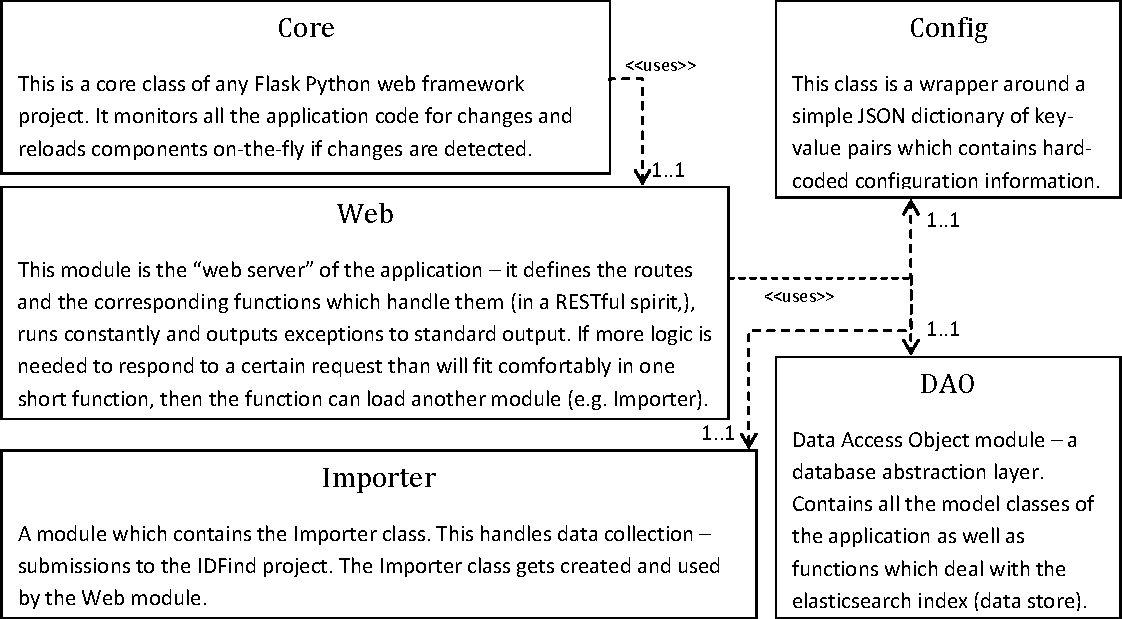
\includegraphics[width=1.00\textwidth,]{idfind-uml.pdf}
\caption{UML diagram of relevant IDFind classes which will become FundFind's classes as more logic is added so that it can actually be called a different project.}
\label{fig:idfind-uml}
\end{figure}


%If your project has a customer, what meetings or interactions have you had so far? If there have been meetings, what did you discuss and will this guide aspects of your project?
\subsection{Customer interaction - ensuring value}
% 1. what the audience is, how much of it is covered, established contacts / meetings
% 2. realised that the audience involved could be wider, contacted or preparing to contact
% 3. how customer interaction ties in with measuring the success of the project

One of the most important aspects to consider when planning a project, selecting a software development methodology and so on is the audience of potential users (``customers'', ``stakeholders'').

\subsubsection{Potential audience}
\label{audience}
The potential audience of this project was discovered to be quite varied:
\begin{enumerate}
	
	\item People looking for funding:
	\begin{itemize}
		\item accomplished scholars (i.e. academics - lecturers, professors)
		\item more ``junior'' academics such as Postgraduate candidates / students and Research Associates
		\item research development officers (professionals who find more funding opportunities for scholars)
	\end{itemize}
	
	\item People looking to advertise funding opportunities. Funding and Programme managers at various institutions such as:
	\begin{itemize}
		\item the Research Councils in the UK
		\item JISC (digital infrastructure in education/research) \cite{jisc}
		\item various charitable Foundations, Institutes, Endowments and so on which fund scholarly activities (e.g. the Wellcome Trust \cite{wellcome-trust}, Shuttleworth Foundation \cite{shuttleworth-foundation}, Knight Foundation \cite{knight-foundation}). Anybody who wants to spend money on scholarship.
	\end{itemize}
	
	\item There is a group which has markedly different needs from the first two groups - people interested in analysing how scholarly money is allocated and/or spent:
	\begin{itemize}
		\item software developers, journalists and others interested in Open Knowledge and visualising data for the purposes of transparency or advancing the digital economy \cite{okfn-vision}
		\item politicians, analysts, bloggers
		\item the general public
	\end{itemize}
\end{enumerate}

\subsubsection{Focusing on certain audience groups}
\label{focus-groups}
Satisfying the major requirements of all these users is not a suitable scope for this project (it may be for a follow-up project).

Therefore, this project will focus on the first group of users. The main reasons are time constraints and ease of access to such users. Searching for opportunities can be significantly harder than submitting them. In a way, providing data to academic users will pave the way for providing data to a more general public (third group) for re-use and analysis.

The project will nonetheless provide basic information submission (``digestion'') capabilities and basic general raw data access via an open machine-ready interface (``API'') to satisfy some of the requirements of the second and third groups. The author belongs to the third group. The Open Knowledge Foundation \cite{okfn-vision} and Cottage Labs LLP \cite{cl} will be briefly consulted on the completed project. Cottage Labs has stated that the project will be valuable to Open Knowledge if executed well and is happy to provide feedback.

\subsubsection{Project constraints due to audience characteristics}
\label{audience-constraints}
All these user groups are professionals. This project is not being developed for a specific client - the time users can dedicate is very limited. As a general rule, user engagement (meetings, e-mail) will stay below 30 minutes per month per user.

\subsubsection{Audience involvement due to audience characteristics}
Since the potential audience is so large, this project will work with:
\begin{itemize}
	\item a Humanities scholar - awaiting response
	\item Science, but not Social or Computer sciences - awaiting response
	\item Computer Science (in addition to supervisor) - accepted
	\item Supervisor - accepted
	\item non-scholars (less regular meetings) - Cottage Labs LLP - accepted
\end{itemize}

All scholars work at Aberystwyth University.

\subsubsection{Measuring success}
This project includes regular releases and evaluation by users as part of its iterative development methodology so that it can demonstrate gradually increasing value. However, towards the end of the development phase there are two weeks dedicated to final, slightly longer evaluation meetings.

Success will be measured by comparing the provided feedback to the final version of the aims of the project. The chosen development methodology harnesses changing requirements to provide more value.

\subsection{Potential issues and risks}
\subsubsection{Potential legal issues}
%Exposing user-submitted data about scholarly funding opportunities to human and machine users could be a problem if the user who submitted the data does not want it to be exposed to others. There are two potential solutions: 
%
%\begin{enumerate}
%	\item force everybody who wants to use the website to open up the data they're submitting (or use another, potentially commercial and proprietary tool).
%	\item allow the specification of licence information when data is submitted to the project (or ingested automatically via web crawling or e-mail digest parsing). Then take the licence into account when exposing the data to anybody.
%\end{enumerate}
%
%The huge potential risk with \#2 is that items are mislabeled, especially by an automated ingestion process, and then the licence terms are breached. The way around this is to only ever run automated processes on data which has clear, blanket Open licensing \cite{od}.
%
%This project goes with \#2, which is more complex, but allows users to use the software to make and manage a private list of funding sources. This way the data is at least present, and an ``Open this up!'' option could be presented to the users.
%
%The other legal issue is setting the software up to parse and understand e-mail digests with funding opportunities meant for human scholarly users. The terms and conditions of each funding organisation will have to be carefully checked, or the organisation will simply have to be contacted directly before such automated e-mail parsing is done.

A possible legal issue the feature which will parse and understand e-mail digests with funding opportunities meant for human scholarly users. The terms and conditions of each funding organisation will have to be carefully checked, or the organisation will simply have to be contacted directly before such processing is done.

\subsubsection{Technical issues}
% 1. enumerate issues and what risk each one represents
% 2. provide risk mitigation strategy for each one
The greatest risk to building software is a bad estimate of how much time it will take, which in turn is notoriously difficult to estimate well.

In this project, the integration of the back-end and front-end technologies could take longer than the allocated week. Spike work on the Javascript visualisation libraries or parsing e-mail digests with funding opportunities could take longer than anticipated.

This project has two general risk mitigation strategies:
\begin{enumerate}
	\item Reordering: during each iteration, do spike work before starting to write tests followed by documentation and code. If the spike work does not seem to make good progress, drop the feature to the end of the queue.
	\item Early value: The main requirements of the software (collecting and presenting data to humans) rely on readily available components to function. These simply have to be brought together with slight modifications - this is the first feature. The software should still be quite valuable to users even if all but that first feature are dropped.
\end{enumerate}


\subsection{Planning progress}
A software development methodology has been chosen and the initial planning phase (as it fits in the chosen methodology) has been completed. Furthermore, suitable project management tools have been chosen and the current plan has been filled in.

\subsubsection{Project management tools}
% mention project management and source code version control as well as server setup
\label{pm-tools}
A project management piece of software suited for Agile approaches was chosen to manage this project: PivotalTracker. The project's progress and an ordered list of features to be developed is publicly available at \cite{pm}. It is recommended that the reader finishes the Planning section of this report before accessing this list since PivotalTracker uses a lot of development methodology-specific terms.

A private source code version control repository was set up with GitHub \cite{github}. This will be made public when it is decided what licence will be used for the software output of the project and the code is of sufficient quality to be publicly released, towards the end of the project.


%==============================================================================
\section{Planning}
%==============================================================================
% 1000 words, 333 words per subsection

Planning methods, techniques and the shape of a project's timeline are usually influenced by the chosen development methodology (or mix of methodologies). The methodology also influences activities around the project - for example, more regular meetings with users (or, by convention, ``customers'') fit the spirit of Agile methodologies.

\subsection{Development methodology}
% 333 words
%say why this needs to be first - planning methods and techniques often follow from the development methodology. It also influences other things around the project like admin e.g. Agile may require more meetings with customers.
%''If you have chosen an agile approach, discuss how this is reflected in your plan, for example thinking about the stories that will be tackled in the different iterations.''

\subsubsection{Considered methodologies}
Development methodologies which were considered include Waterfall \cite{waterfall}, V-shaped model \cite{vmodel}, double-V model (a.k.a. W-model) \cite{wmodel}, spiral model \cite{spiral-model}, Behaviour-Driven Development \cite{bdd}, Feature-Driven Development \cite{fdd}.

\subsubsection{Chosen methodology}
\label{chosen-dev}
This project has adopted an Agile approach to both its software and documentation development (including the final report). There is a great variety of Agile practices and some are better suited for groups of developers, so certain well-known examples like Pair Programming \cite{pairprg} or full Scrum \cite{Scrum} were found to be unsuitable.

The reasons were varied, but generally included Agile's advantage when it comes to capturing fluctuating user requirements over time. Another advantage is the apparent ease of communication - the user does not have to provide a full functional specification of what they want, they can use more vague descriptions in the form of ``stories'' which describe the feature(s) they want \cite{stories}. It is worth noting that Feature-Driven Development is also an agile approach but is more suitable for larger projects. Behaviour-Driven Development is an interesting idea, but requires more effort / time on the users' side (the need to learn a domain-specific language).

Requiring less customer time (see \S\ref{audience-constraints})and exploiting a very lean project management and development methodology is particularly important in this project. With this and the Agile Manifesto \cite{agile-manifesto} in mind, a methodology of an Agile character was laid out, using the Extreme Programming lifecycle as a base \cite{xp-lifecycle}. 

The length of one iteration will be one week. Considering the tight deliverable deadlines (see \S\ref{timeline}), this will keep work on the project focused and will force the definition of user stories of a manageable size.

%Agile approaches usually \emph{avoid} defining ``size'' - how long it will take to implement a story. Rather the complexity of each story is estimated using \emph{arbitrary} numbers (some people prefer to use larger/smaller animals) - how difficult it is to implement that story relative to other stories. If a story seems too \emph{complex}, it needs to broken up. This project uses the Fibonacci number sequence \cite{fibonacci} and ``too complex'' is a complexity estimate of more than 3. Previous experience with the technologies involved has also helped provide a link between complexity and ``how much time will it take'', thus helping enforce a maximum of 1 week to complete a story and add value to the software.

The basic steps are:
\begin{enumerate}
	\item Meet with a variety of potential users from the chosen user group (\S\ref{focus-groups}), trying to pick them so that each one has a different professional perspective on scholarship.
	\item Define \emph{and prioritise} the functionality of the project with each user in the form of the ``stories'' mentioned above. Record the results using the chosen project management tools (\S\ref{pm-tools}).
	\item Release planning - prepare an initial timeline of which project features are to be released when and denote ``release points''. This work can be repeated as required - the order and the features themselves might change on the basis of user feedback over time (this is how Agile projects try to deliver more value by responding to changing requirements). The total size of the work and the size of each feature will most probably remain the same. This piece of work produces the ``Project Timeline'' and the current version is included in \S\ref{timeline}.
	\item Iterate - every week is a self-contained unit of work consisting of coding, documentation and write-up work. Before starting to code each week, break up that week's story into tasks so goals can be tracked more effectively and there is something to be accomplished each day.
	\item Repeat items 1 and 2 - meaning regular meetings with previously chosen users - one per user per month, demonstrate the latest features and record the feedback.
\end{enumerate}

Within the coding part of each iteration, Test-Driven Development is employed using both unit and integration tests (the latter via browser automation with Selenium \cite{selenium}). This will be the evidence (on a basic technical level) for the ``correctness'' of the software. A basic form of Continuous Integration \cite{ci} will also be used - the Jenkins \cite{jenkins} software is currently being evaluated for the job. It basically runs all automated tests continuously, helping to detect regressions in code quality.

This methodology makes for a considerably simpler lifecycle than the Extreme Programming one (a visualisation of which can be accessed at \cite{xp-lifecycle}). This is intentional as there are only about 11 (potentially 13) weeks which allow for programming work as can be seen in \S\ref{timeline}.

\newpage

\subsection{Current project timeline}
\label{timeline}
% provide explanations (and include in chart) missing weeks like holidays, exams. Mention I'm not doing job interviews BUT I am working extracurricularry so..
% explain how I'm doing write-up alongside code

\begin{figure}[H]
\centering
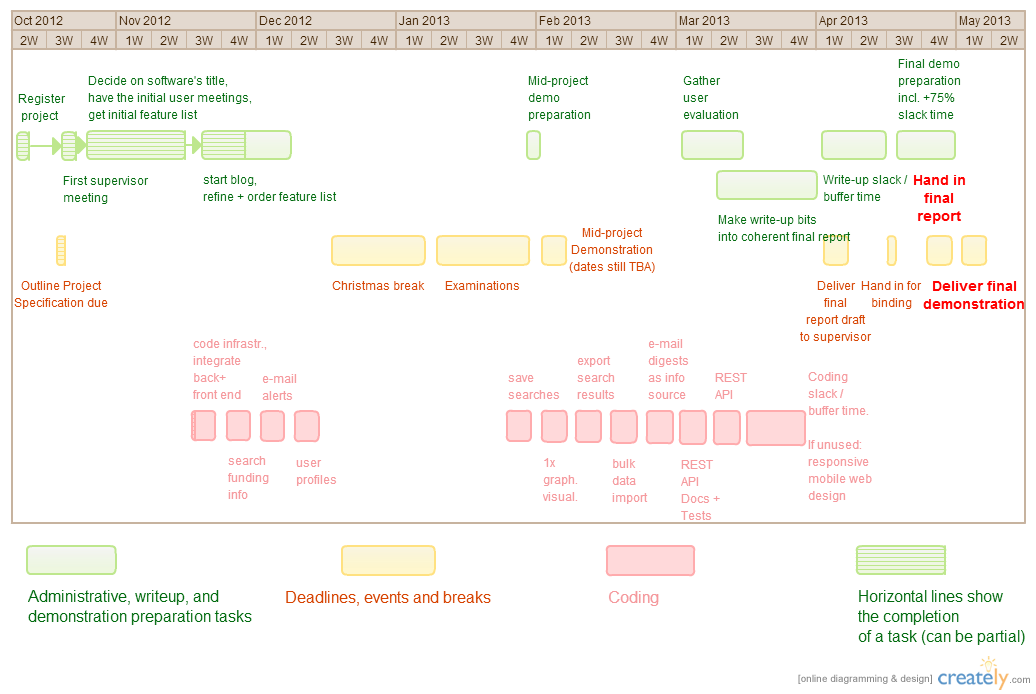
\includegraphics[height=0.6\textheight,angle=90]{timeline.png}
\caption{FundFind project timeline}
\label{fig:timeline}
\end{figure}

Figure \ref{fig:timeline} visualises the current project timeline. It is being referred to as the ``current'' one since the order of or the actual features being implemented could change due to the Agile project development methodology, as described in \S\ref{chosen-dev}. There could also be other factors which might influence the order of implementation of features, such as implementing ``flashier'' features slightly earlier than the users' feedback dictates - for example, before the Mid-project demonstration. ``Flashy'' means producing easily recognisable valuable output such as summaries and graphical visualisations.

The latest list of features with longer descriptions and more information than the timeline Gantt chart can be accessed at \cite{pm}.

It should be noted there are necessary chores which do not add value to the software. Examples: publicly hosting the project; project management tasks; writing reports such as this one. This is reflected in the following breakdown of the 400-hour time budget:

\subsubsection{Time budget breakdown}
\label{time-budget}
% also include my 400h breakdown (will need to expand more into what I've done in October!)
% demos are part of ``admin''
Available in Table \ref{tab:time-breakdown}.

\begin{table}[H]
\centering
\begin{tabular}{p{2cm}|p{6cm}|c|>{\centering}p{2cm}<{\centering}|c}
	Type of activity & Activity & Repetition & Time (1 occurence) & Total time \\
	\hline
	discussion & 5x (Nov-March) regular meetings with 4 users & 20 & 0.5h & 10h \\[3pt]
	discussion & Supervisor meetings & 23 & 0.5h & 11.5h \\[3pt]
	discussion & E-mail / talk to Cottage Labs / OKFN & 4 & 0.25h & 1h \\[3pt]
	production & Project Outline Specification & 1 & 3h & 3h \\[3pt]
	production & Progress report & 2 & 6h & 12h \\[3pt]
	production & Mid-project demonstration & 4 & 1h & 4h \\[3pt]
	production & Write-up (ongoing through lifetime of project) & 92 & 1h & 92h \\[3pt]
	production & Final demonstration & 4 & 2h & 8h \\[3pt]
	admin & Project management & 30 & 1h & 30h \\[3pt]
	production & Software development & 200 & 1h & 200h \\[3pt]
	buffer & Slack available if any of these tasks take longer than estimated & N/A & N/A & 28.5h \\[3pt]
	\hline
	meta & Total project time & N/A & N/A & 400h \\
\end{tabular}
\caption{Project time budget}
\label{tab:time-breakdown}
\end{table}

\subsection{Demonstrating value}
% 333 words for whole subsection, 150 words intro paragraph, 90 words per demo
% introduction paragraph to this subsection

% demos: plan to show fully working version of the app with some valuable features, in the spirit of the chosen dev. methodology

No special equipment or software will be necessary on the demonstration computer for both of the demonstrations, just a relatively modern graphical web browser.

Preparatory work for both demonstrations includes making sure that:
\begin{enumerate}
	\item application is running in a publicly visible location
	\item the Continuous Integration tool is working and all tests are passing
	\item there is enough data loaded into the application to demonstrate more complex features such as faceted search \cite{faceted}
	\item the application works as intended in the web browser(s) on the demonstration computer
\end{enumerate}

The project will be demonstrated as a fully working application in both demonstrations (although user feedback could have altered the feature list). The timeline \S\ref{timeline} shows which features are currently planned for completion before(therefore inclusion into) each demonstration.

\subsubsection{Mid-project demonstration}
The first demonstration will show a ``less valuable'' version of the software with basic capabilities for collecting funding data and searching through it. Currently, the timeline also includes one basic graphic visualisation as a feature for this demonstration.

\subsubsection{Final demonstration}
The final demonstration will include all of the features in the timeline (subject to the usual Agile user feedback influence).

The RESTful API will be demonstrated using a small Python web application which will try to get the data exposed via the API and output details to the screen. The API documentation will then be shown on screen and brief comments on the API's conformity to RESTful principles will be made.

%If the responsive mobile web design is included (it is currently allocated to the ``optional'' coding time at the end of the coding phase), it will be demonstrated using screenshots from an emulator service such as Browshot \cite{browshot}. It may also be demonstrated on one real mobile device - this is not guaranteed, however, since the author does not currently own any mobile devices with modern mobile web capabilities.

%
% Start to comment out / remove the following lines. They are only provided for instruction for this example template.  You don't need the following section title, because it will be added as part of the bibliography section. 
%
%==============================================================================
%\section*{Your Bibliography - REMOVE for final version}
%==============================================================================
%
%You need to include an annotated bibliography. This should list all relevant web pages, books, journals etc. that you have consulted in researching your project. Each reference should include an annotation. 
%
%The purpose of the section is to understand what sources you are looking at.  A correctly formatted list of items is sufficient. You might go further and make use of bibliographic tools, e.g. BibTeX in a LaTeX document, could be used to provide citations, for example \cite{NumericalRecipes} \cite{MarksPaper} \cite[99-101]{FailBlog} \cite{kittenpic_ref}.  The bibliographic tools are not a requirement, but you are welcome to use them.   
%
%You can remove the above {\em Your Bibliography} section heading because it will be added in by the renewcommand which is part of the bibliography. The correct annotated bibliography information is provided below. 
%
% End of comment out / remove the lines. They are only provided for instruction for this example template. 
%


\nocite{*} % include everything from the bibliography, irrespective of whether it has been referenced.

% the following line is included so that the bibliography is also shown in the table of contents. There is the possibility that this is added to the previous page for the bibliography. To address this, a newline is added so that it appears on the first page for the bibliography. 
\newpage
\addcontentsline{toc}{section}{Annotated Bibliography} 

%
% example of including an annotated bibliography. The current style is an author date one. If you want to change, comment out the line and uncomment the subsequent line. You should also modify the packages included at the top (see the notes earlier in the file) and then trash your aux files and re-run. 
%\bibliographystyle{authordate2annot}
\bibliographystyle{IEEEannot}
\renewcommand{\refname}{Annotated Bibliography}  % if you put text into the final {} on this line, you will get an extra title, e.g. References. This isn't necessary for the outline project specification. 
\bibliography{mmp} % References file


\end{document}